% ADRC speed controller with Extended State Observer.
% Compile: pdflatex speed-loop-adrc.tex && pdf2svg ...
\documentclass[tikz, margin=4mm]{standalone}
\usetikzlibrary{arrows.meta, positioning, calc}

\tikzset{
  block/.style = {draw, rectangle, rounded corners=2pt, align=center,
                  fill=blue!8, font=\small,
                  minimum height=1.0cm, minimum width=2.8cm},
  sum/.style   = {draw, circle, fill=blue!8, minimum size=7mm, inner sep=0pt},
  arr/.style   = {-{Latex[length=4pt, width=5pt]}, thick},
  lbl/.style   = {font=\footnotesize},
  node distance = 0.9cm and 1.8cm
}

\begin{document}
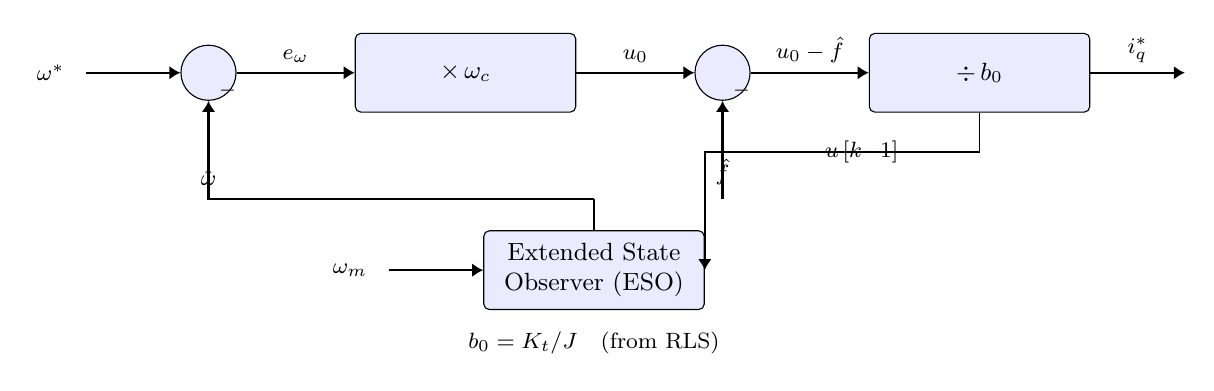
\begin{tikzpicture}

  % ── Control law (top path) ────────────────────────────────────────────────
  \node[sum]                           (Sw)     {};     % ω* − ω̂
  \node[block, right=1.5cm of Sw]      (Kc)     {$\times\,\omega_c$};
  \node[sum,   right=1.5cm of Kc]      (Sdf)    {};     % u0 − f̂
  \node[block, right=1.5cm of Sdf]     (Div)    {$\div\, b_0$};

  % ── Extended State Observer ───────────────────────────────────────────────
  \node[block, below=2.0cm of $(Kc)!0.5!(Sdf)$]
        (ESO) {Extended State\\ Observer (ESO)};

  % ── I/O ───────────────────────────────────────────────────────────────────
  \coordinate (WrefIn) at ($(Sw.west)+(-1.2,0)$);
  \coordinate (IqOut)  at ($(Div.east)+(1.2,0)$);
  \coordinate (WmIn)   at ($(ESO.west)+(-1.2,0)$);

  % ── Connections ───────────────────────────────────────────────────────────

  % Reference
  \node[lbl, left=0.15cm of WrefIn] {$\omega^*$};
  \draw[arr] (WrefIn)  -- (Sw);

  % u0 path
  \draw[arr] (Sw)  -- node[lbl,above]{$e_\omega$} (Kc);
  \draw[arr] (Kc)  -- node[lbl,above]{$u_0$}       (Sdf);
  \draw[arr] (Sdf) -- node[lbl,above]{$u_0 - \hat{f}$} (Div);
  \draw[arr] (Div.east) -- node[lbl,above]{$i_q^*$}  (IqOut);

  % Measured speed to ESO
  \node[lbl, left=0.15cm of WmIn] {$\omega_m$};
  \draw[arr] (WmIn) -- (ESO);

  % u feedback to ESO
  \coordinate (Ufb) at ($(Div.south)+(0,-0.5)$);
  \draw (Div.south) -- (Ufb);
  \draw[arr] (Ufb) -| node[lbl,right,pos=0.3]{$u\,[k{-}1]$} (ESO.east);

  % ESO estimates → control law
  \coordinate (ESOtop) at ($(ESO.north)+(0,0.4)$);
  \draw (ESO.north) -- (ESOtop);

  % ω̂ to summing junction (negative)
  \coordinate (WhatJoin) at (ESOtop -| Sw);
  \draw[arr] (ESOtop) -- (WhatJoin)
             -- (Sw) node[below right, font=\scriptsize]{$-$};
  \node[lbl, above=0.05cm of WhatJoin] {$\hat{\omega}$};

  % f̂ to feedforward cancellation summing junction (negative)
  \coordinate (FhatJoin) at (ESOtop -| Sdf);
  \draw[arr] (FhatJoin) -- (Sdf) node[below right, font=\scriptsize]{$-$};
  \node[lbl, above=0.05cm of FhatJoin] {$\hat{f}$};

  % b0 label
  \node[lbl, below=0.15cm of ESO] {$b_0 = K_t/J$\quad (from RLS)};

\end{tikzpicture}
\end{document}
